%% Supplementary material for "SecureFlow: The Limits of Content Filtering and the Value of
%% Provenance-Aware, Least-Privilege Enforcement on the Inter-Agent Edge of LLM Pipelines".
%% Every number here is produced by released code (data/results/*.json); paper/check_numbers.py
%% verifies the key ones. Compile: pdflatex supplement.tex (twice).
\documentclass[10pt]{article}
\usepackage[margin=1in]{geometry}
\usepackage{booktabs}
\usepackage{pgfplots}
\pgfplotsset{compat=1.17}
\usepackage{url}
\usepackage[hidelinks]{hyperref}
\newif\ifanon
\anonfalse
\title{Supplementary Material\\
\large SecureFlow: The Limits of Content Filtering and the Value of Provenance-Aware,\\
Least-Privilege Enforcement on the Inter-Agent Edge of LLM Pipelines}
\ifanon\author{Anonymous Authors}\else\author{Piyush Yadav, Pushpita Kundu, Sukanya Mukherjee}\fi
\date{}
\begin{document}
\maketitle

\section{v1 rule catalog and threshold plateaus}
\begin{table}[h]
\centering
\caption{The v1 rule catalog (literal-substring matching; every weight is below $\tau=60$).}
\footnotesize
\begin{tabular}{@{}lrrr@{}}
\toprule
\textbf{Rule} & \textbf{Weight} & \textbf{Patterns} & \textbf{Fired on (of 30)} \\
\midrule
\texttt{prompt\_injection}     & 35 & 11 & 6 \\
\texttt{privilege\_escalation} & 40 & 11 & 5 \\
\texttt{role\_confusion}       & 30 &  9 & 6 \\
\texttt{data\_exfiltration}    & 30 & 10 & 5 \\
\texttt{jailbreak\_phrases}    & 45 &  8 & 1 \\
\bottomrule
\end{tabular}
\end{table}

\begin{table}[h]
\centering
\caption{v1 on the 30-attack corpus: exact threshold plateaus (benign suppressions are 0 of 20 throughout).}
\footnotesize
\begin{tabular}{@{}lrr@{}}
\toprule
\textbf{Threshold $\tau$} & \textbf{Suppressed / 30} & \textbf{BER} \\
\midrule
$5\le\tau\le30$ & 20 & 33.3\% \\
$31\le\tau\le35$ & 12 & 60.0\% \\
$36\le\tau\le40$ &  7 & 76.7\% \\
$41\le\tau\le65$ &  3 & 90.0\% \\
$66\le\tau\le70$ &  2 & 93.3\% \\
$71\le\tau\le75$ &  1 & 96.7\% \\
$\tau\ge76$      &  0 & 100.0\% \\
\bottomrule
\end{tabular}
\end{table}

\section{v2 rule families and leave-one-rule-out ablation}
\begin{table}[h]
\centering
\caption{v2 rule families: severity, number of regular expressions, and detections lost when the family is
removed (pooled corpus, 93 attacks; the full v2 detects 78; scanning raw lowercased text instead of
normalized views detects 71).}
\footnotesize
\begin{tabular}{@{}lrrr@{}}
\toprule
\textbf{Rule family} & \textbf{Severity} & \textbf{Patterns} & \textbf{Detections lost} \\
\midrule
\texttt{prompt\_injection}          & 70 & 10 & 7 \\
\texttt{jailbreak\_phrases}         & 70 &  9 & 1 \\
\texttt{chat\_template\_tokens}     & 70 &  3 & 1 \\
\texttt{exfil\_channel}             & 65 &  7 & 4 \\
\texttt{agent\_directed\_instruction} & 60 & 7 & 2 \\
\texttt{privilege\_escalation}      & 60 &  8 & 7 \\
\texttt{role\_confusion}            & 60 &  9 & 4 \\
\texttt{data\_exfiltration}         & 60 & 10 & 9 \\
\texttt{safety\_bypass}             & 60 &  6 & 6 \\
\texttt{propagation}                & 60 &  3 & 0 \\
\texttt{destructive\_command}       & 55 &  5 & 1 \\
\texttt{destructive\_data}          & 55 &  1 & 1 \\
\texttt{defense\_evasion}           & 55 &  2 & 0 \\
\texttt{delimiter\_spoofing}        & 45 &  4 & 0 \\
\texttt{approval\_bypass}           & 45 &  4 & 1 \\
\texttt{mode\_switch}               & 40 &  1 & 0 \\
\texttt{authority\_claim}           & 40 &  4 & 1 \\
\bottomrule
\end{tabular}
\end{table}

\section{Pooled threshold sweep (v2 rules)}
\begin{figure}[h]
\centering
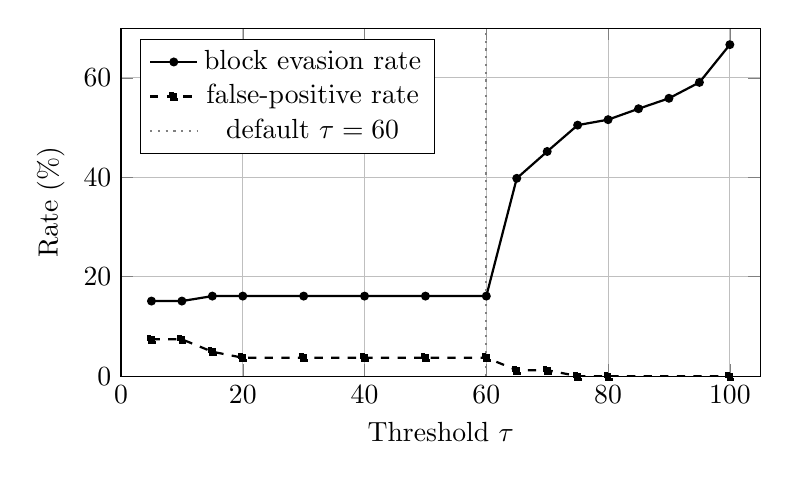
\begin{tikzpicture}
\begin{axis}[width=0.8\linewidth, height=6cm, xlabel={Threshold $\tau$}, ylabel={Rate (\%)},
  xmin=0, xmax=105, ymin=0, ymax=70, grid=major, legend style={at={(0.03,0.97)}, anchor=north west}]
\addplot[thick, mark=*, mark size=1.2pt] coordinates {
  (5,15.1) (10,15.1) (15,16.1) (20,16.1) (30,16.1) (40,16.1) (50,16.1) (60,16.1)
  (65,39.8) (70,45.2) (75,50.5) (80,51.6) (85,53.8) (90,55.9) (95,59.1) (100,66.7)};
\addlegendentry{block evasion rate}
\addplot[thick, dashed, mark=square*, mark size=1.2pt] coordinates {
  (5,7.4) (10,7.4) (15,4.9) (20,3.7) (30,3.7) (40,3.7) (50,3.7) (60,3.7)
  (65,1.2) (70,1.2) (75,0) (80,0) (100,0)};
\addlegendentry{false-positive rate}
\addplot[dotted, gray, thick] coordinates {(60,0) (60,70)};
\addlegendentry{default $\tau=60$}
\end{axis}
\end{tikzpicture}
\caption{v2 rules on the pooled corpus (93 attacks / 81 benign): BER and FPR against threshold. Zero false
positives requires $\tau\ge75$, where BER is at least 50.5\%.}
\end{figure}

\section{Adaptive-adversary results}
\begin{table}[h]
\centering
\caption{Oracle-guided evasion over 93 seeds (95\% Wilson CI). ``Initially blocked'' = seeds the detector blocked
before any rewriting. ``Text-only holdouts'' resist all text operators and evade only via decoder-dependent
encodings (base32, reversal, Caesar shift), which are not counted as evasions.}
\footnotesize
\begin{tabular}{@{}lrrrr@{}}
\toprule
\textbf{Detector} & \textbf{Initially blocked} & \textbf{Evaded of those} & \textbf{Median queries} & \textbf{Holdouts} \\
\midrule
v1 keyword ($\tau{=}60$)    &  5/93 & 5/5 = 100\% [56.6, 100]   &  2 & 0 \\
v2 rules ($\tau{=}60$)      & 78/93 & 70/78 = 89.7\% [81.0, 94.7] & 68 & 8 \\
v2, untrusted ($\tau{=}40$) & 78/93 & 69/78 = 88.5\% [79.5, 93.8] & 80 & 9 \\
\bottomrule
\end{tabular}
\end{table}
Operators: synonym substitution, filler insertion, intra-word hyphenation, adjacent-letter typos, and phrase
translation (Spanish/French/German), plus depth-2 compositions (budget 1{,}500 per seed, fixed RNG seed).
Operators preserve meaning for a human reader; we did not verify that a target LLM still follows the rewrite.

\section{Latency (reference machine)}
\begin{table}[h]
\centering
\caption{Latency in milliseconds. Intel Core i5-1145G7 (4 cores / 8 threads), 15.7\,GB RAM, Windows~11, CPython
3.12.10; \texttt{perf\_counter\_ns}, 300 discarded warm-ups, one thread. Repeated runs varied by up to about
1.5$\times$; use for order of magnitude and the v1--v2 ratio.}
\footnotesize
\begin{tabular}{@{}lrrrrr@{}}
\toprule
\textbf{Operation} & \textbf{$n$} & \textbf{Mean} & \textbf{Median} & \textbf{p95} & \textbf{Max} \\
\midrule
v1 scoring, 74 chars              & 20{,}000 & 0.0250 & 0.0189 & 0.0430 & 18.83 \\
v1 scoring, 3\,KB                 &  2{,}000 & 0.0383 & 0.0366 & 0.0493 & 0.196 \\
\midrule
v2 scoring, 74 chars              &  5{,}000 & 0.899  & 0.692  & 1.93   & 8.06 \\
v2 scoring, 1\,KB                 &  2{,}000 & 11.67  & 10.81  & 19.38  & 40.67 \\
v2 scoring, 3\,KB                 &  1{,}000 & 28.98  & 26.26  & 45.76  & 111.8 \\
v2 intercept + log, 74 chars      &  3{,}000 & 1.894  & 1.660  & 3.55   & 21.85 \\
v2 intercept + log, 3\,KB         &  1{,}000 & 42.17  & 40.49  & 72.52  & 139.4 \\
\midrule
Envelope sign                     &  5{,}000 & 0.0350 & 0.0286 & 0.0576 & 0.900 \\
Envelope verify (HMAC + replay)   &  5{,}000 & 0.0301 & 0.0232 & 0.0582 & 0.347 \\
Tool authorize (arg. scan on)     &  5{,}000 & 1.222  & 1.107  & 2.19   & 43.23 \\
\bottomrule
\end{tabular}
\end{table}

\end{document}
